\item \points{2b} Now add a regularization term to your cross entropy loss by implementing |backward_prop_regularized()|.
The loss function will become \begin{equation*}
  J_{MB} = \left(\frac{1}{B}\sum_{i=1}^{B}CE(y^{(i)}, \hat{y}^{(i)})\right) + \frac{1}{2} \lambda \left(\vert \vert W^{[1]}\vert \vert ^2 + \vert \vert W^{[2]}\vert \vert ^2 \right)
  \end{equation*}

Autograder test case |2b-2-basic| will perform the same as |2aii-6-basic| (described earlier), except that it utilizes your new regularized backprop function.  Before running this test case, edit line 285 of |src-mnist/grader.py| to state |skip = False| (model plotting/training is disabled by default to run the auotgrader faster).  It will also plot the same
figures as part (a). Note that it does NOT include the regularization term to measure
the loss value for plotting (i.e., regularization should only be used for gradient calculation for
the purpose of training).

\clearpage\newpage
After creating the plots from the previous part, they should look similar to the following (You are not required to submit any plots.  These are for your own verification.):

\begin{figure}[H]
    \centering
    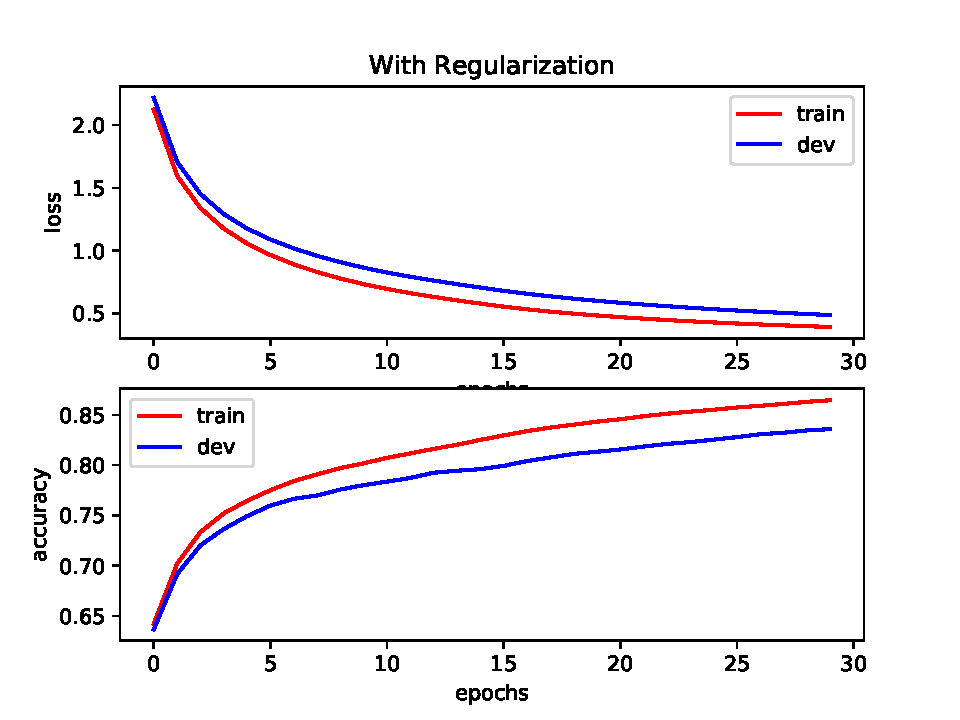
\includegraphics[scale=0.75]{02-mnist/regularized.pdf}
\end{figure}
